% 
% %\documentclass[paper=a4,fontsize=12pt,open=right,noabbrev]{report}
% \documentclass[12pt]{report}
% \usepackage[utf8]{inputenc}
% \usepackage{amsmath}
% \usepackage{amssymb}
% \usepackage{graphicx}
% \usepackage{placeins}
% \usepackage{cite}
% \usepackage{physics}
% \usepackage{mathrsfs}
% \usepackage{geometry}
% % \usepackage{layouts}
% \usepackage{newfloat}
%  \usepackage{float}
% 
% \setlength{\parindent}{0em}
% \setlength{\parskip}{1em}
% 
% 
% %% Technical point floatstyle
% \floatstyle{ruled}
% \newfloat{Technical Point}{htbp}{lop}[chapter]
% 
% 
% \begin{document}

\chapter{Reweighting Dynamics in full Conformational Space }
\label{ch:RewU}

 
This chapter focuses on testing the reweighting scheme introduced in section~\ref{sec:RewOffEqu} on minimal models where the full conformational space is known. We have seen in chapter~\ref{ch:Jaynes} that the chosen set of constraints apply for a test model. We extend this testing by variation of of  potentials, dimension and magnitude of local and global forces. The models consist of a single particle so entropic effects due to many-body interactions are absent. This provides a minimal testing ground for the reweighting method based on the Maximum Caliber. At first, an equilibrium model with changing potential surface is test for the special case of equilibrium systems. The second systems extends to non-equilibrium steady states (NESS) by a global external force with periodic boundary conditions, introduced in section~\ref{sec:1Dmodel}. The third system is inspired by a laser model and pushes the system in a NESS by applying non-conservative forces locally~\cite{khan1983mechanism}. The last model adds one dimension and tests the global driving on a 2-dimensional single particle. 

The systems are simulated using molecular dynamics for 10 different driving forces and a Markov State Model (MSM) is constructed. One system is reweighted continuously to other thermodynamic state points and checked if dynamical and static information from simulation are recovered correctly. The static information is tested using the stationary distribution, the dynamical information is tested using the first-passage-time distribution (FPTD) between metastable states (see section~\ref{sec:FPTD}). Selected processes are compared by full FPTD, because comparison of all FPTD with each other is cumbersome. The systems are compared by the first three moments of the FPTD and the metastable state occupation probabilities $\Pi$. The reweighting test is considered successful if all information is recovered correctly.

The presented results for all models except the 2D model were published in~\cite{bause2019microscopic}.


\section{Single Particle in 1D Potential Well}
\label{sec:equ}
\begin{figure}[h]
\centering
 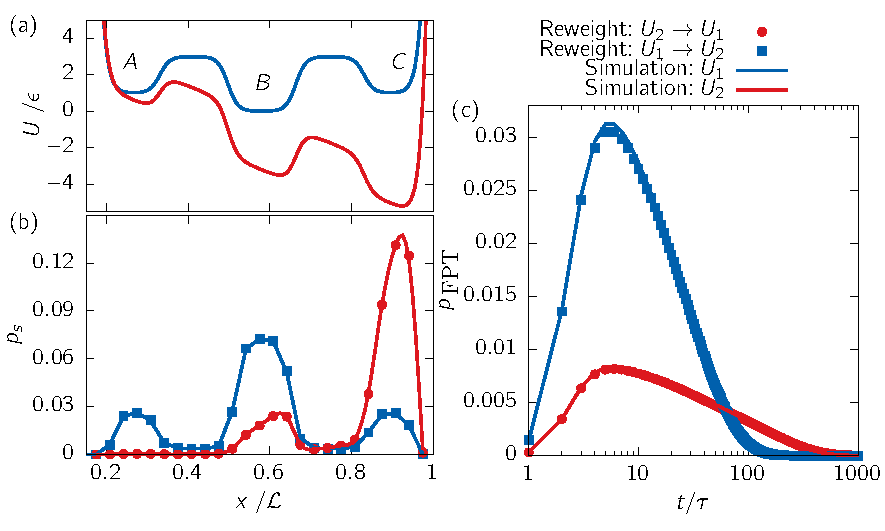
\includegraphics{../plots/Urew/single_3003.pdf}
 \caption[Potential surface, stationary distribution and first-passage time distribution of a chosen process for the 1D equilibrium system]{ (a) Potential, (b) stationary distribution and (c) FPTD of the process $ C \rightarrow B$. The lines in (b,c) represent the results from simulating the system potentials, the dots are the results from reweighting the systems into each other. $A$, $B$, $C$ mark the metastable states. The system without tilting is represented blue, the system with tilting in red. }
 \label{fig:potequ} 
\end{figure}

The reweighting procedure is designed for general NESS. We will test it on the special case of an equilibrium model first. The potential shown in figure~\ref{fig:potequ} is a 1D potential of a type presented in section~\ref{sec:1Dmodel} with diverging boundaries and three potential wells. 
The applied force in positive direction can be described by an additional potential $U_{\text{ext}}(x) = -f x $ that tilts the existing potential. The diverging boundaries prevent the system to enter a NESS and restrict the system to equilibrium. Equilibrium is a case of a NESS without entropy production on average and the dynamics are governed by detailed balance. It ensures that the heat dissipated moving a particle between two points in space does not depend on the chosen trajectory. The MSM was constructed with a lagtime $0.004\,\mathcal{T}$ and $60$ microstates. 
 
The static and dynamic properties for the system without potential tilt and with maximum tilting at $f= 9\,\frac{\epsilon}{\mathcal{L}}$ are shown in figure~\ref{fig:potequ}. The presented FPTD from state $C$ to $B$ slows down significantly with increasing tilting. Transition times above $50\,\tau$ are rare in the reference system and become likely in the new potential. The reweighting procedure recovers this detailed view on the dynamics. Previously unknown trajectories are captured by the reweighting correctly. 
\begin{figure}
\centering
 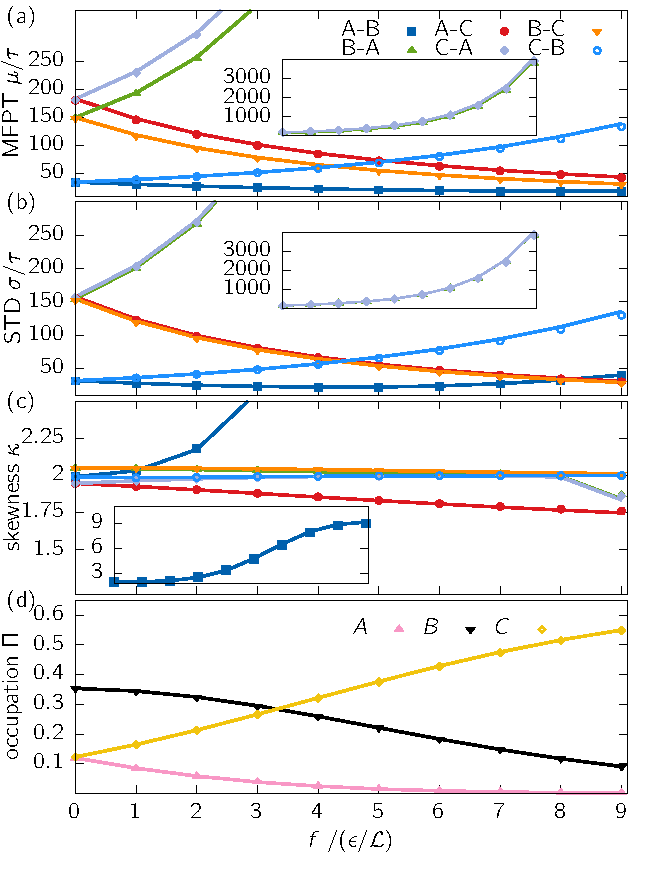
\includegraphics{../plots/Urew/mom_3003.pdf}
 \caption[The first three moments and the population of metastable states for the equilibrium system under varying tilt of the potential.]{$(a-c)$ The first three moments of the FPTD for all six processes between metastable states in figure~\ref{fig:potequ}a under varying tilting of the potential. $(d)$ The occupation probability of each metastable state. The dots represent the value measured from simulation. The line is the equilibrium system continuously reweighted.  }
 \label{fig:momequ}
\end{figure}

Figure~\ref{fig:momequ} presents the first three moments and the occupation probability of the metastable states. The potential is constructed such that two processes have the same FPTD in equilibrium: $A \rightarrow B$ and $C \rightarrow B$ going from left and right inwards to the central potential, their inverse processes going outwards from the central potential and processes $A \rightarrow C$ and $C \rightarrow A$. The latter processes  crossing the whole system via state $B$ and can be seen as a combination of two processes. The additional force breaks the symmetry and speeds up the processes in the direction of the force, while inverse processes are slowed down. The standard deviation (STD) of the distributions show the same behavior as the mean first-passage time (MFPT). A larger mean allows larger variation. The skewness is  stable at $\approx 2 $, except for the process $A \rightarrow B$. This process is increasingly fast, such that it is described by processes of time-length of the lagtime $\tau$, as shown in figure~\ref{fig:potequ}c. The fast processes cannot be described in all detail anymore, resulting in a tilting of the distribution and an increasing skewness. Smaller lagtime of the MSM would shift this effect to higher driving forces.  

Reweighting continuously from the equilibrium system shows the precision of the method over the range of driving forces. Furthermore, the driven states between the simulated ones can be explored without additional simulation. It is concluded that the reweighting method recovers static and dynamic properties from reweighting for the special case of equilibrium systems. We will turn to the general class of all NESS in the next section.



\FloatBarrier
\section{Single Particle in 1D under Global Driving}
\label{sec:1gl}
\begin{figure}[h]
 \centering
 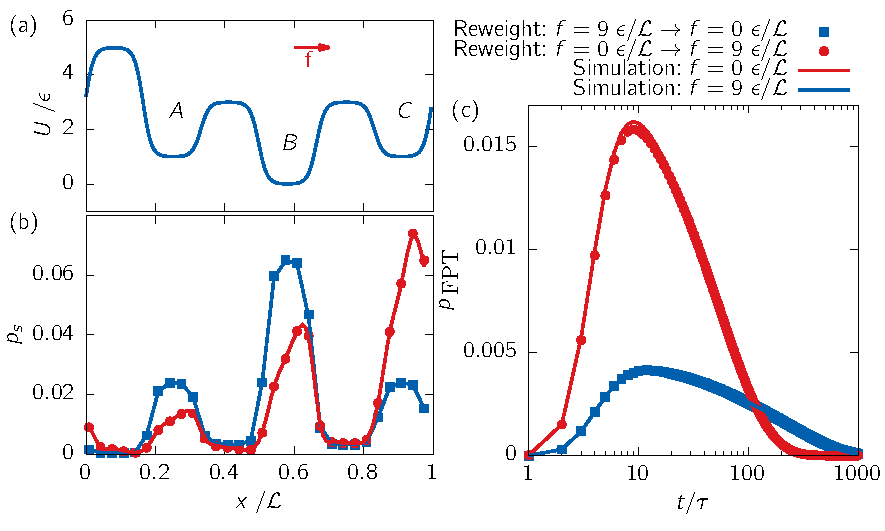
\includegraphics{../plots/Urew/single_2010.pdf}
 \caption[Potential surface, stationary distribution and first-passage time distribution of a chosen process for the 1D driven system]{ (a) Potential and external force (b) stationary distribution and (c) FPTD of the process $ C \rightarrow B$. The lines in (b,c) represent the results from simulating a single particle in the potential without (blue) and with (red) external force. The dots are the results from reweighting the systems into each other. $A$, $B$, $C$ mark the metastable states. }
 \label{fig:potgl}
\end{figure}

A single particle in 1D periodic-boundary potential is driven in one direction by an external force. Since the particle has a preferred direction to move the dynamics do not fulfil detailed balance. The external force cannot be described by a potential. The heat dissipated to move the particle between two space-points becomes path-dependent. In particular, the heat  dissipated depends on weather the particle moving between two points in space along a trajectory with or against the external force. The present model is a minimal example to describe a NESS. The reweighting scheme will be shown to capture the path-dependence of the dynamics correctly.

The corresponding MSM describing the dynamics is constructed from simulation data in detail in section~\ref{sec:MSM} with a lagtime $\tau = 0.002\,\mathcal{T}$ and $60$ microstates. The reference potential surface with non-conservative forces is shown in figure~\ref{fig:potgl}a. The diverging potential at the boundaries of the equilibrium system in the previous section~\ref{sec:equ} was replaced  by a potential barrier of height $5\,\epsilon$. The stationary distribution and a FPTD for a chosen process without driving and a system driven by $9\, \frac{\epsilon}{\mathcal{L}}$ are shown in figure~\ref{fig:potgl}b,c. The systems are reweighted into each other. The simulation and reweighting data match precisely for the stationary distribution and the FPTD from state $C$ to $B$. 

\begin{figure}[t]
\centering
 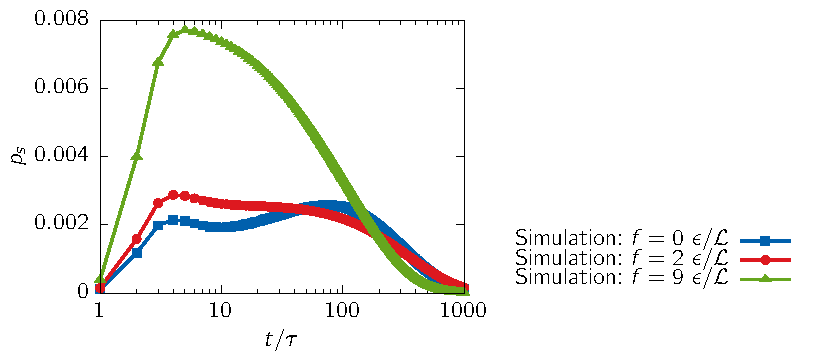
\includegraphics{../plots/Urew/fpt_2010.pdf}
 \caption[First-passage time distribution of transition $C\rightarrow A$ simulated at 3 different driving forces for the 1D driven system.]{FPTD of transition $C\rightarrow A$ simulated at 3 different driving forces. The equilibrium system at $f=0$ is a bimodal distribution, indicating two sets of trajectories for that trajectory. The two peaks merge to one as driving increases. One set of trajectories is suppressed by the driving.  }
 \label{fig:fpt1D}
\end{figure}

The potential shown in figure~\ref{fig:potgl}a represents the equilibrium system without driving force.  The direction of the force is marked in red and applied over the whole system with equal strength. The first three moments of the FPTD for all involved slow processes and the stationary distribution of metastable states is shown in figure~\ref{fig:momgl}. The processes $A\rightarrow B$ and $B\rightarrow C$ are aligned with the external force and become faster. The process $C\rightarrow A$ shows abnormal behaviour by slowing down first and speeding up at force $> 4\,\frac{\epsilon}{\mathcal{L}}$. For the reference system, the connection via state $B$ is spatially longer but more probable than the direct connection over the large barrier. Both sets of trajectories are presented by two peaks in the FPTD in figure~\ref{fig:fpt1D}. This weighting of path changes under driving until the jump over the large barrier between the states becomes more probable for increasing driving. At this point, the process speeds up with increasing force. The process $B\rightarrow A$ opposing the external force slows down first. After the jump over the barrier between state $A$ and $C$ becomes more probable, the transition  $B\rightarrow A$ benefits from using new transition trajectories via state C and increases speed. The transition $C\rightarrow B$ slows down against the force. We can expect that the trend changes for larger forces too.  The STD show a similar behaviour as the MFPT as seen for the previous system. The skewness is more variable, but stays in a range of $\approx 2 $. The skewness of transition $A\rightarrow B$ increases due to its strong increase in short-term processes, as described for the previous system in section~\ref{sec:equ}. The increase is less than for the previous system, because a lower lagtime for the MSM was chosen. The occupation probability changes over driving such that state $B$ becomes higher populated than state $C$ for driving $> 4\,\frac{\epsilon}{\mathcal{L}}$. This \textit{population inversion} is an off-equilibrium effect where population of high energy states is larger than the population of low energy states~\cite{maes2018non}. It cannot exist in equilibrium because populations follow Boltzmann statistics. 

The current minimal system shows complex non-equilibrium behaviour by introducing path-dependence.  This path-dependence of transition breaks the monotonous increase/decrease in MFPT under driving from the equilibrium system by promoting one collection path over another. This is not possible in equilibrium systems. Additionally population inversion is achieved by breaking detailed balance: A probability flow from one state of the system is allowed without a symmetric back-flow, irrespective of the stationary distribution. Global balance makes sure that the probability flows away in other direction so probability flow is conserved. 

The presented method shows perfect results for the case of NESS. We will continue by testing the boundaries of the driving and the effect of local driving on the reweighting procedure. 

\begin{figure}
\centering
 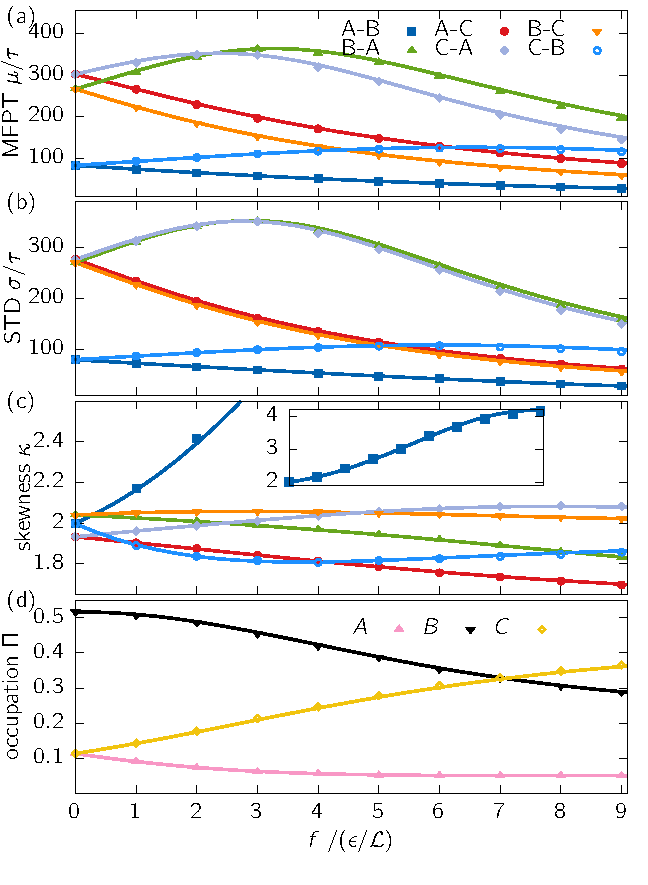
\includegraphics{../plots/Urew/mom_2010.pdf}
 \caption[The first three moments and the population of metastable states for the 1D driven system for varying external force.]{(a-c) The first three moments of the FPTD for all six processes between metastable states in figure~\ref{fig:potgl}a under varying external force $f$. (d) The occupation probability of each metastable state. The dots represent the value measured from simulation. The line is the equilibrium system continuously reweighted.  }
 \label{fig:momgl}
\end{figure}
\FloatBarrier

\section{Single Particle in 1D under Local Driving}
\label{sec:Lasersys}
\begin{figure}[h]
\centering
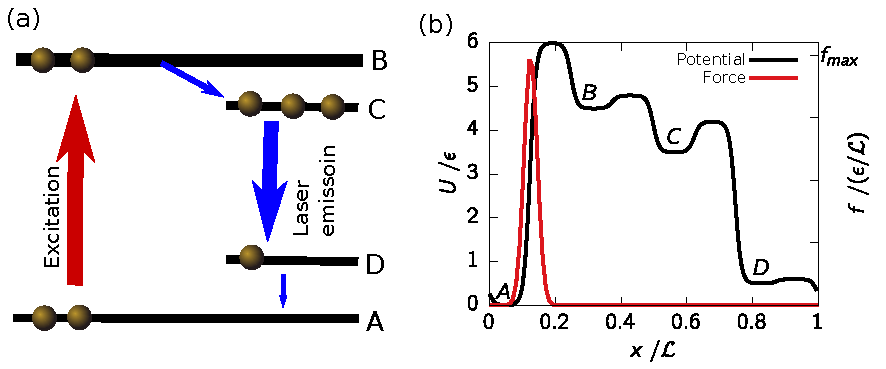
\includegraphics{../images/laser.pdf}
\caption[Sketch of a 4-state laser model with potential surface and pumping force.]{ (a) Sketch of a 4-state laser model. The electron are pumped from state $A$ to state $B$, marked by the red arrow. The blue arrows represent relaxation transition. The transition $C \rightarrow D$ relaxes under emission of a photon. (b) Translation of laser model to a continuous potential surface. The excitation is represented by a Gaussian force in the direction of the potential barrier.  }
\label{fig:laser}
\end{figure}

\begin{figure}[t]
\centering
 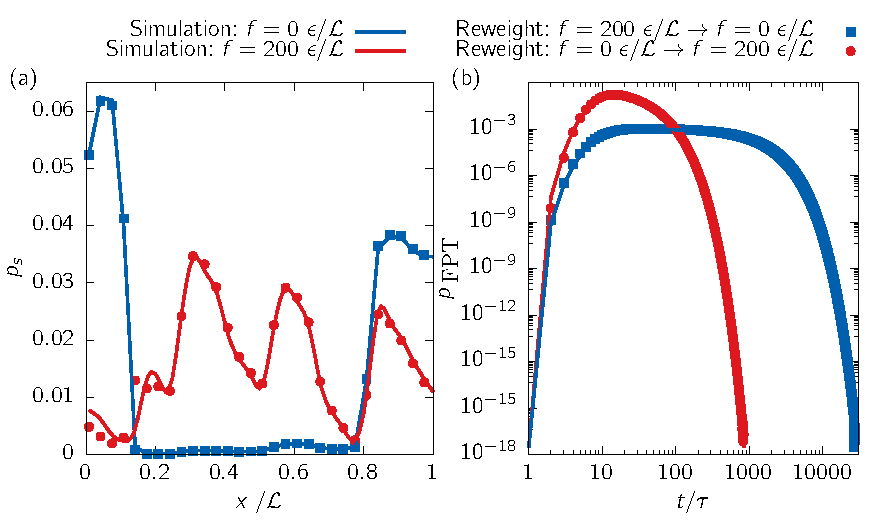
\includegraphics{../plots/Urew/single_9040.pdf}
 \caption[Stationary distribution and first-passage time distribution of the excitation process for the laser model.]{(a) stationary distribution and (b) FPTD of the excitation process $ A \rightarrow B$. The lines in (a,b) represent the results from simulating a single particle in the potential without (blue) and with (red) external force. The dots are the results from reweighting the systems into each other. }
 \label{fig:singleL}
\end{figure}

This model is inspired by a laser model with 4 states. A laser is in a far-off-equilibrium steady state and shows population inversion where high energy electron states are more populated than low energy states~\cite{kaschke2013optical}. Relaxing electrons from the high energy state to a low energy state emits photons. The steady state is driven by an external force pumping  electron to higher energetic states. The laser starts emitting monochromatic light when the higher energy states are more  populated than the lower states. 

An electron in figure~\ref{fig:laser} starting in state $A$ is pushed to the highest energetic state $B$ by external driving. Typically, the energy is provided by optical illumination and photon absorption, chemical reactions or electronic discharge~\cite{kaschke2013optical}. In this simplified model, the driving is represented by a Gaussian shaped force irrespective of the source. From the highest state, it relaxes fast to a state $C$ with slightly lower energy under emission of heat in form of vibrations to surrounding atoms. This state is used to depopulate state $B$, so it can be repopulated quickly by the pumping. The electron relaxes from state $C$ to $D$  by emitting a photon. In practice the emission may happen by spontaneous or stimulated emission. The  relaxation from state $D$ to $A$ is fast under the emission of vibrational energy to surrounding atoms like the transition $B \rightarrow C$. 
The depopulation of state $D$ will promote the desired transition $C \rightarrow D$. Direct transitions between non-neighbouring states like $B \rightarrow D$ are forbidden by the selection rules of quantum mechanics. All described transition may occur the other way round by random fluctuations. The pumping will promote the described path and suppress the inverse path. Without this pumping, the forward and backward transition becomes equally likely, i.e. the system fulfils detailed balance and Boltzmann statistics apply. The flow in cycles is essential for a NESS. That means a 3-state laser model can be constructed by deleting supporting states $B$ or $D$ and it can show population inversion too. A 2-state laser would automatically fulfil detailed balance and cannot show population inversion.

The model is not designed to be an accurate presentation for a laser. The helium-neon-laser for example uses 3 states of the helium and 6 states of the neon gas~\cite{leach2014fundamental}. The number of states, the barriers and energy levels are chosen purely phenomenological. The transition states are modelled by a steep potential slope and the classical Langevin equation does not represent quantum mechanical transitions. There is only a single particle in the system, i.e. the electron is non-interacting. The model is designed to achieve a complete population inversion, where the equilibrium occupation order is inverted for all four states. It shows that the equilibrium and driven states share less dynamics than in the previous 1D system. The reweighting procedure requires reliable reference data, so this model is challenges it by the absence of common dynamics. Furthermore, the reweighting procedure is challenged by external forces that act locally.

The MSM was constructed with $64$ microstates and a lagtime of $0.002\,\mathcal{T}$. The equilibrium system and a system driven at peak force $200\,\frac{\epsilon}{\mathcal{L}}$ is compared in figure~\ref{fig:singleL}. It should be noted that the peak force is 20 times larger than external forces used in previous systems.  The stationary distribution is recreated well by the reweighting procedure. There is a small artifact at the peak of the external force for the reweighted driven system. The FPTD is shown for the pumped transition from $A$ to $B$. The short-time processes are more probable by a factor of 10 for the pumped process compared to the equilibrium process. The equilibrium system shows transition over the whole spectrum from $10$ to $10000$ Markovian steps. The reweighting procedure recovers the FPTD for both systems although transition times differs by a factor of 10. 

The comparison for different driving forces by the first three moments of the FPTD and the metastable state population is shown in figure~\ref{fig:momL}. The analysis shows the pumping and emission transition and their corresponding inverse transition. Note the logarithmic scale in MFPT and STD to capture the large differences in timescales of the observed systems. The MFPT of the pumping transition $A \rightarrow B$ speeds up drastically as desired. The inverse transition opposing the pumping is affected much less and the mean increases slowly. The duration of the desired relaxation transition $C \rightarrow D$ is unaffected by the pumping. However, the transition is happening more frequently because state $C$ is much higher populated than in equilibrium. The inverse relaxation $D \rightarrow C$  speeds up with the pumping  caused by the cyclic motion via $A$ and $B$, not by a direct jump. Again, the STD follows the behaviour of the mean, also in magnitude. The skewness does not show any new behaviour, the skewness of transition $A \rightarrow B$ is increasing when approaching low MFPT. The stationary distribution shows the first population inversion of state $B$ and $C$ for $ f> 70\,\epsilon / \mathcal{L}$. The populations are globally inverted for $f > 170\,\epsilon / \mathcal{L}$.

Simulation and reweighting from equilibrium agree well, but some deviation can be seen for increased driving. Major deviations occur in the MFPT and the skewness of the NESS of transition $A \rightarrow B$ for driving $f >\,150 \epsilon / \mathcal{L}$. The MFPT is underestimated due to the defect in stationary distribution shown in figure~\ref{fig:singleL}a. This deviation can be an effect of the discretisation of state. The localised Gaussian force is continuous in simulation and discretised in the reweighting procedure, where it spreads out over just a few microstates in the MSM. The local error does not effect other transitions.  The reweighting procedure can capture localised forces but the microstates should be chosen fine so the discretised description of the forces is sufficient. Most of the deviations occur when the driving is very large compared to previous driving forces. The large deviation in skewness is connected to the same effect for very low MFPT described for the previous systems. The method relies on sufficient data from the reference simulation. The underlying dynamics of both processes are so different that deviations can occur because the reference sampling is noisy, similar to the effect of missing reference data in equilibrium reweighting (see section~\ref{sec:rewEqu}).  Furthermore, the MSM was constructed for the reference system. The dynamics of the driven system are much faster and the lagtime can be too large to describe the system properly.   Considering these effects, deviations for heavy driving are in an acceptable range. 


We achieved the desired total population inversion as a limitation test for the reweighting procedure. It shows that far-off equilibrium phenomena are captured by the reweighting, despite the approximation close to detailed balance for a single jump. The construction of long trajectories from single transitions marginalises the error.  The effect of local forces was tested in depth. The model demonstrates that local entropy productions are essential for NESS, a global constraints would not be able to capture the local driving in this model. 


\begin{figure}
\centering
 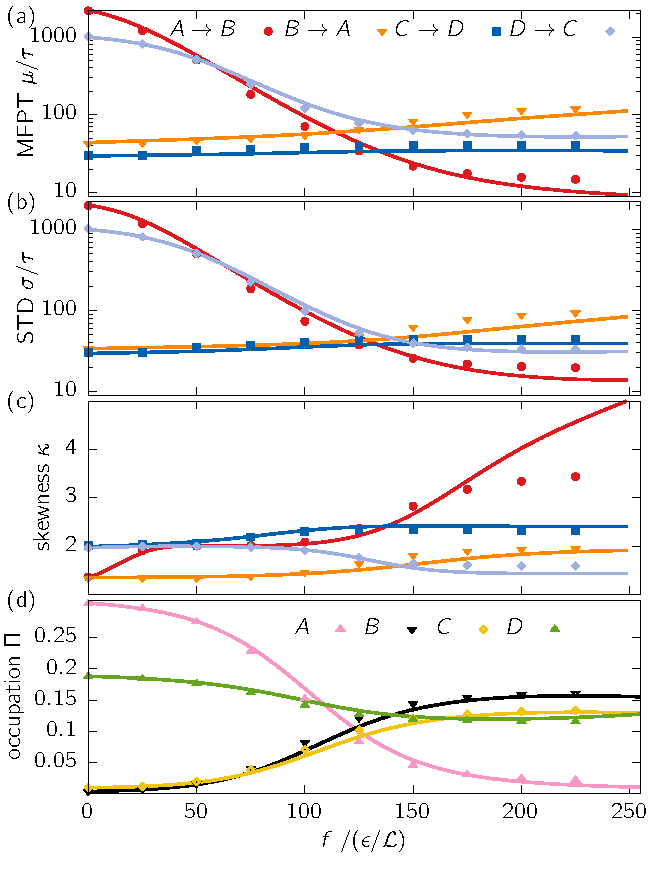
\includegraphics{../plots/Urew/mom_9040.pdf}
 \caption[The first three moments and the population of metastable states for the laser system for varying external force.]{(a-c) The first three moments of chosen FPTD between metastable states in figure~\ref{fig:singleL} under varying external force $f$. The transition are the pumping transition $A \rightarrow B$ and the emission transition $C \rightarrow D$ with both inverse transitions. (d) The occupation probability of each metastable state. Full population inversion for driving $f >\,170 \epsilon / \mathcal{L}$.  The dots represent the value measured from simulation. The line is the equilibrium system continuously reweighted. }
 \label{fig:momL}
\end{figure}
\FloatBarrier

\section{Single Particle in 2D under Global Driving} 
\label{sec:2Dsys}

\begin{figure}
\vspace{-0cm}
\centering
 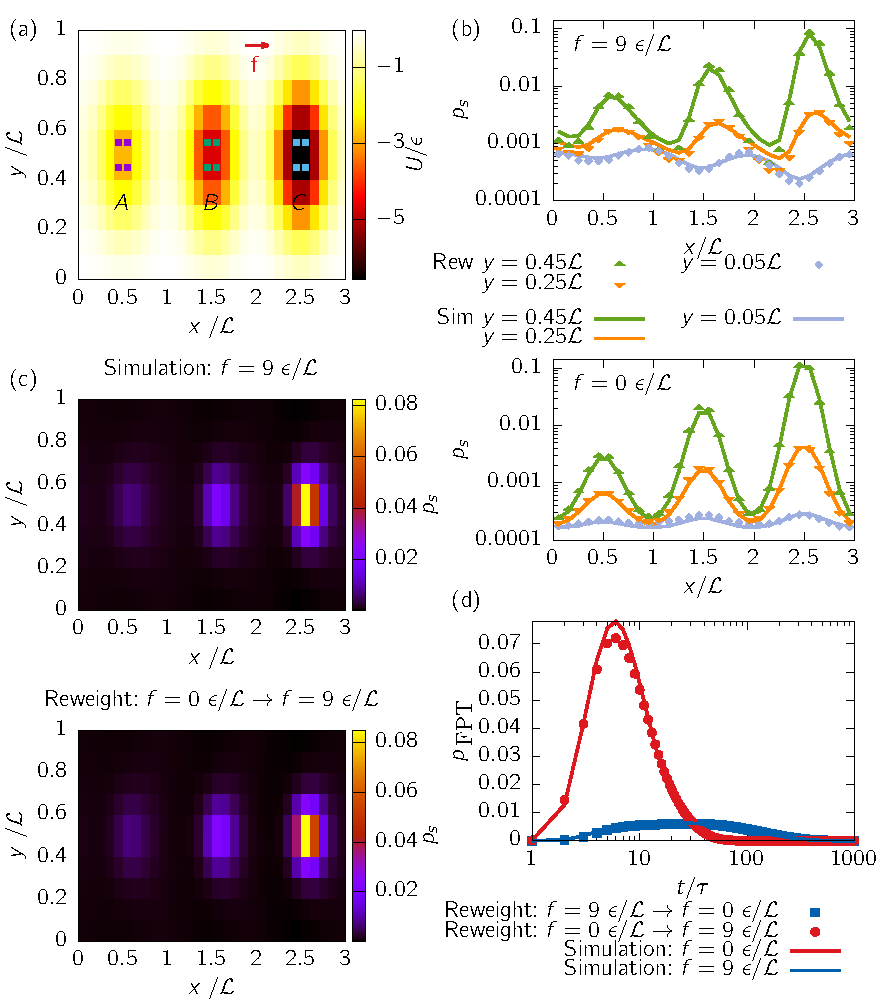
\includegraphics{../plots/Urew/single_5010.pdf}
 \caption[Potential surface, stationary distribution and first-passage time distribution of a chosen process for the 2D driven system]{(a) The potential surface with the metastable states marked $A$, $B$, $C$. (b) Stationary distribution under driving from simulation and from reweighting. (c) Detailed view on the stationary distribution in equilibrium and driven with $9\,\frac{\epsilon}{\mathcal{L}}$ on states with $y=0.05\,\mathcal{L}, 0.25\,\mathcal{L}, 0.45\,\mathcal{L}$. The lines are the results from simulation, the dots from reweigthing into each other. (d) FPTD of the process $ C \rightarrow B$. The lines represent the results from simulating a single particle in the potential without (blue) and with (red) external force. The dots are the results from reweighting the systems into each other.  }
 \label{fig:pot2D}
\end{figure} 

The non-interacting particle is suspended in a 2D potential to introduce a second degree of freedom that has to be recovered correctly. The configuration space increases quadratically and challenges the reweighting method by a large number of microstates. 

The potential consists of three Gaussian potential wells of varying depth, shown in figure~\ref{fig:pot2D}a. All boundaries are periodic and the external force is applied along the $x$-direction. The microstates consists of $30$x$10$ squares of equal size, the lagtime was chosen at $0.02\,\mathcal{T}$. The potential minima were chosen at $3\,\epsilon$, $5\,\epsilon$ ,and $7\,\epsilon$, located on a line in the middle of the y-axis. The STD of the Gaussian is $0.02\,\mathcal{L}$ in both directions.    

A detailed view on the stationary distribution is given in figure~\ref{fig:pot2D}c. The simulated system at $9\,\frac{\epsilon}{\mathcal{L}}$ and the reweighted system agree in probability distribution at first sight. Figure~\ref{fig:pot2D}b adds the probabilities distribution for $(i)$ a $y$-value along the middle of the system, $(ii)$ one at boundary of the system and $(iii)$ one in the middle of these two, comparing the simulated and reweighted stationary distribution.  The probability density around the minima decreases with driving and more states surrounding the minima are occupied. Within the basins, the distribution is tilted in the direction of the force. Turning to the result of reweighting, the logarithmic scale reveals a deviation when reweighting from equilibrium to the driven system. The error is smaller reweighting vice versa. The occupation probabilities between the basins are estimated too low and in the minima too high. This error was not identified for the 1D-systems and it is more pronounced in the driven than in the equilibrium system. Turning to figure~\ref{fig:pot2D}d the FPTD of the transition $C \rightarrow B$ peaks at faster processes for the driven system because the transition via $A$ becomes more prominent. The equilibrium transitions occur at a broader probability peaking between $10\,\tau-30\,\tau$.  A small deviation between simulation and reweighting can be seen at the peak of the driven distribution. The process speeds up by a factor of $10$.    
\begin{figure}
\centering
 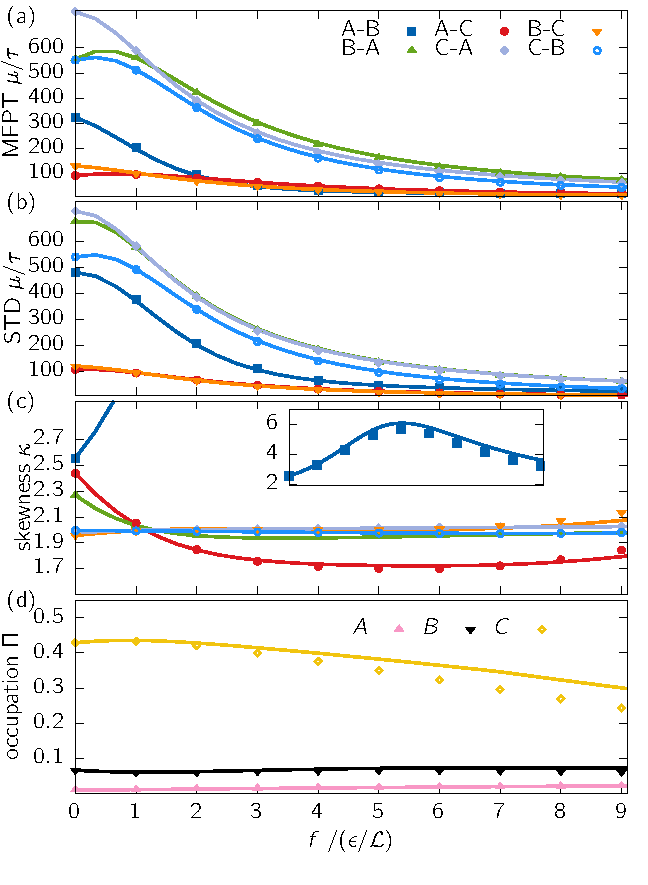
\includegraphics{../plots/Urew/mom_5010.pdf}
 \caption[The first three moments and the population of metastable states for the 2D system for varying external force.]{ (a-c) The first three moments of the FPTD for all six processes between metastable states in figure~\ref{fig:pot2D}a under varying external force $f$. (d) The occupation probability of each metastable state. The dots represent the value measured from simulation. The line is the equilibrium system continuously reweighted. }
 \label{fig:mom2D}
\end{figure}

The first three moments of the six slowest FPTD and the metastable state occupation probability is shown in figure~\ref{fig:mom2D}. The MFPT becomes faster for all processes under driving. Only the processes $C \rightarrow B$ and $B \rightarrow A$ slow down for small driving before speeding up. Similar to the 1D system in section~\ref{sec:1gl}, this can be explained by an initial slowing down by the particles taking the direct path against the force. For larger driving the spatially longer paths along the external force become more prominent and increase speed of the process. Compared to the 1D system under global driving, this phenomena comes into effect for much lower driving although the potential barriers are larger.  A possible reason is the bypassing of the intermediate state because the potential barriers are small close to the $y$-boundaries. The increase in occupation probability in $y$-direction supports this argument, because more trajectories pass by these states. Again, the STD shows the same trend as the MFPT. The skewness levels $\approx 2$ again. The process $A \rightarrow B$ shows abnormal behaviour in skewness by increasing until $4\,\frac{\epsilon}{\mathcal{L}}$ and then decreasing again. The skewness of process $A \rightarrow C$ on the other hand becomes smaller than than for the other processes, indicating a tilting of the distribution to the right. Both effects can be explained with another set of slower processes entering the system for increasing driving: The potential in $A$ is a too weak obstacle for the particle flowing by.
\begin{figure}[t]
\centering
 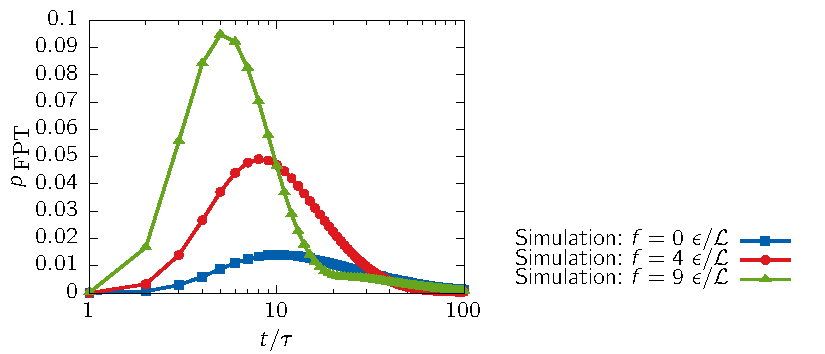
\includegraphics{../plots/Urew/fpt_5010.pdf}
 \caption[First-passage time distribution of transition $A \rightarrow B$ simulated at 3 different driving forces for the 2 system.]{FPTD of transition $A \rightarrow B$ simulated at 3 different driving forces. Increased driving promotes short-time processes and suppresses slow processes. For $f =9\,\frac{\epsilon}{\mathcal{L}}$ a second peak appears at $\approx 30\,\tau$, showing new long-term processes.  }
 \label{fig:fpt2D}
\end{figure}
There is an increasing probability that they simply bypass the metastable state lying in the minimum of the potential and produce trajectories longer than the system size. The effect is shown in figure~\ref{fig:fpt2D} where increased driving results in an increase of short-time processes in $A \rightarrow B$ on the left-hand-side of the distribution. Further driving produces a second small peak on the right-hand-side, showing the long-time processes bypassing $A$. The decrease in MFPT is slowing down and the skewness  decreases by this effect. The bypassing can only occur for a 2D system.  The metastable state occupation in figure~\ref{fig:mom2D} of state $C$ decreases and occupation of state $A$ and $B$ stay approximately the same. The depopulation of the highest probability state was seen in the 1D system too. The other states do not increase in population because the probability generally spreads out from the potentials minima. A broader definition of metastable states would capture this in an increase of occupation probability with increasing driving. The reweighting procedure has problems capturing the true magnitude of $C$ as discussed earlier in the detailed view on the stationary distribution in figure~\ref{fig:pot2D}. 

The reweighting technique shows excellent results for this model too. We can see some deviation, e.g. for the peak of the FPTD in figure~\ref{fig:pot2D}d or the occupation probability between the basins in figure~\ref{fig:pot2D}b. Both effects only take place when reweighting over a broad range of driving. The additional degree of freedom requires a larger number of microstates and defines a challenge for the reweighting procedure and gives insight in its possible limitations. In particular we find that states away from the basins are not recovered correctly by the reweighting. The sources of deviation for all systems will be discussed in detail in the next chapter. 



\FloatBarrier
\section{Discussion}
The previous sections applied the reweighting scheme to a number of different systems, all being single particles in different external potentials under varying driving forces. The potential surface and the external forces can be varied locally once an MSM for a reference system is created. The gathered information can be reweighted to any other system, as long as it is similar to the reference system. This section discusses the precision and limitation of this method.

The method needs two sets of input data: Any reference data in form of an MSM and the local entropy production of the target system. The latter can be included by the total entropy production $\Delta S_{ij}$ from state $i$ to $j$ or by the difference in entropy production of reference and target system $\Delta S_{ij} - \Delta S^q_{ij}$ as shown in equation~\ref{eq:finalpij}. Any system can be chosen for a reference, indicating that there is an underlying invariance in the reference systems, as it was introduced in equation~\ref{sec:Invariant}. This consequences of the invariant is further discussed in section~\ref{sec:InvariantC}. 

The method relies on sampling transition probabilities of a system sufficiently. The underlying simulated trajectories give a more detailed picture but are broken into pieces of local transitions. Sampling the transition probabilities is a much easier task than sampling complete trajectories. As a result trajectories that do not exist in the reference system are constructed by the MSM of the reweighted system. This can be seen in the FPTD for all systems (see figure~\ref{fig:potequ}, \ref{fig:potgl} , \ref{fig:singleL}, \ref{fig:pot2D}). The underlying MSM allows us to construct trajectories that are important in the target system. This is a fundamental difference to the Ferrenberg-Swendsen reweighting for equilibrium introduced in section~\ref{sec:rewEqu}: The method fails if states required in the target system are not sufficiently sampled in the reference system. Translated to dynamics, it means that the important transition probabilities of the target system have to be sampled sufficiently in the reference system. The complete trajectories do not need to overlap because they can be constructed afterwards. The locality of the entropy productions is key for the system to work because each part of the trajectory is reweighted individually to constitute the local nature of non-equilibrium processes. The global balance condition account for the interaction of all microtransition.

The MFPT and the STD of the FPTDs show similar trend and magnitude for all systems. Exponential distribution have the property $\sigma = \mu$. The large tails of the FPTDs decay exponentially and dominate the variance of the system. The observed values for mean and STD become  similar for our systems but not equal because they deviate from exponential distributions for short time processes.  

\subsection{Sources of Error}
\label{sec:Error}
The FPTD shows small deviations from its expected distribution with increasing reweighting distance. This deviation is largest in the peaks of the FPTD distribution and for the stationary distribution of the 2D system in figure~\ref{fig:mom2D}. Error analysis was performed on different systems to exclude sampling issues. Other sources of the deviation are possible and are discussed in the following:

\begin{itemize}
 \item The approximation was used in the deviation of the reweighting formula
 \item Insufficient constraints in the Maximum Caliber
 \item Chosen microstates and lagtime of reference MSM might be unsuitable for target system
 \item Limitation for large fluctuations
\end{itemize}

The necessity of the approximation was discussed in detail in section~\ref{sec:numerics}. The exact set of equations emerging from the Caliber cannot be solved numerically. Furthermore the full set of equation may have more than one solution and it cannot be guaranteed to find the correct one. The approximation solves this issue by having a singular solution and fulfilling the constraints of the Caliber. The significance of this error cannot be determined without an available full solution. 
 
Constraining the Caliber according to the local entropy production is based on how the system interacts with its environment. Global balance is introduced to model the internal connection of the states. Success of the method is based on the quality of the constraints. It cannot be excluded that other effects play a major role. If other effects exist they are minor for the given systems. If new constraints can be identified it can be included in the Caliber in form of Lagrangian multipliers. For now we assume the set of constraint to be complete.

Another source of error is based on the construction of the Markov State Model. The microstates are chosen equi-sized and independent of data so all models can be represented by it. The lagtime on the other hand is chosen based on a method  requiring equilibrium data (see section~\ref{sec:MSM}). The method fails for NESS, so the lagtime of the reference equilibrium system is assumed to be valid for the target system too. When reweighting over large distances this assumption might be flawed. An indicator is the MFPT that changes considerably e.g. for the laser system. This suggests a change in timescale and the lagtime of the target MSM might be chosen inconsistent with the Markovian assumption. The user has to reweight MSMs constructed at different lagtimes to check for deviations based on this issue. 

\begin{Technical Point}[tp]

\begin{minipage}{0.03\textwidth}
\hfill\vspace{0.1cm}
\end{minipage}%
\begin{minipage}{0.35\textwidth}
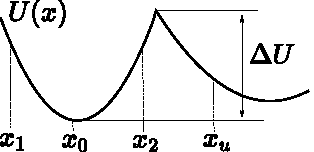
\includegraphics{../images/kramers.pdf}
\end{minipage}
\hfill
\begin{minipage}{0.6\textwidth}
The Kramers model~\cite{kramers1940brownian} describes non-dissipative dynamics of molecular reactions by a 1-dimensional potential $U(x)$ coupled to a head-bath at temperature $T$ with coupling constant $\gamma$. It estimates the rate of a transitioning over a barrier by 
\end{minipage}
\begin{equation*} 
 k = \frac{k_{\mathrm{B} }T}{\gamma} \left ( \int_{x_0}^{x_u} \exp \left ( \frac{U(x)}{k_{\mathrm{B} }T} \right ) \int_{x_1}^{x_2} \exp \left ( \frac{-U(x)}{k_{\mathrm{B} }T} \right )\right )^{-1}
\end{equation*}
The first integral is over the transition region, the second integral captures the starting potential or the initial probability distribution. Kramers showed 
how the transition rate depends on the form and the height of the potential. It requires that the equilibration time $\tau_e$ in one basin is much smaller than the transition times $\tau_t \gg \tau_e$. To be consistent we have to assume that $k_{\mathrm{B} }T \ll \Delta U$.
% 

\caption{The Kramers Model}\label{tec:kramers}
\end{Technical Point} 


The method is limited to systems where fluctuations are not stronger than the potential surface. Tests showed that potential barriers of $ \Delta U < k_{\mathrm{B} }T$ are not captured well by the reweighting method. The random fluctuation takes over the system-dependent local entropy productions.  The barrier crossing dynamics are governed by the local potentials and captured well (see technical point~\ref{tec:kramers}). The diffusion dynamics governed by symmetric fluctuations on the other hand are not well captured. This effect can be seen in the 2D system in figure~\ref{fig:mom2D} where trajectories bypass some potential minima for heavy driving. The potential barrier close to the boundary in $y$-direction is often smaller than kinetic energy from fluctuations. Once these states show larger population, the error becomes more pronounced. The presented errors for heavy driving might emerge from this limitation of the method. 

The mentioned sources of errors are oftentimes difficult to check. However, this chapter shows that the errors are minimal compared to the range of the reweighting method. Even increasing/decreasing the speed of processes by the order of 10 is captured with minor deviation. A full error analysis on the construction of the MSM or developing a maximisation algorithm for the full solution of the Caliber can be useful for future investigation.  The presented data proves the concept of Caliber maximisation under constraining global balance and local entropy production by reweighting MSM between NESS. The proposed combination of constraints form a functional ensemble for NESS at different temperatures, different potentials and various strength and form of driving.    


% % 
% \bibliography{/home/marius/PhD/Thesis/references.bib}
% \bibliographystyle{plain}
% \end{document}
